%%%%%%%%%%%%%%
%% Run LaTeX on this file several times to get Table of Contents,
%% cross-references, and citations.

%% If you have font problems, you may edit the w-bookps.sty file
%% to customize the font names to match those on your system.

%% w-bksamp.tex. Current Version: Feb 16, 2012
%%%%%%%%%%%%%%%%%%%%%%%%%%%%%%%%%%%%%%%%%%%%%%%%%%%%%%%%%%%%%%%%
%
%  Sample file for
%  Wiley Book Style, Design No.: SD 001B, 7x10
%  Wiley Book Style, Design No.: SD 004B, 6x9
%
%
%  Prepared by Amy Hendrickson, TeXnology Inc.
%  http://www.texnology.com
%%%%%%%%%%%%%%%%%%%%%%%%%%%%%%%%%%%%%%%%%%%%%%%%%%%%%%%%%%%%%%%%

%%%%%%%%%%%%%
% 7x10
%\documentclass{wileySev}

% 6x9
\documentclass{wileySix}

\usepackage{graphicx}
\usepackage{listings}

\usepackage{color}
 
\definecolor{codegreen}{rgb}{0,0.6,0}
\definecolor{codegray}{rgb}{0.5,0.5,0.5}
\definecolor{codepurple}{rgb}{0.58,0,0.82}
\definecolor{backcolour}{rgb}{0.95,0.95,0.92}
 
\lstdefinestyle{mystyle}{
    backgroundcolor=\color{backcolour},   
    commentstyle=\color{codegreen},
    keywordstyle=\color{magenta},
    numberstyle=\tiny\color{codegray},
    stringstyle=\color{codepurple},
    basicstyle=\footnotesize,
    breakatwhitespace=false,         
    breaklines=true,                 
    captionpos=b,                    
    keepspaces=true,                 
    numbers=left,                    
    numbersep=5pt,                  
    showspaces=false,                
    showstringspaces=false,
    showtabs=false,                  
    tabsize=2,
    language=sh
}
 
\lstset{style=mystyle}

%%%%%%%
%% for times math: However, this package disables bold math (!)
%% \mathbf{x} will still work, but you will not have bold math
%% in section heads or chapter titles. If you don't use math
%% in those environments, mathptmx might be a good choice.

% \usepackage{mathptmx}

% For PostScript text
\usepackage{w-bookps}

%%%%%%%%%%%%%%%%%%%%%%%%%%%%%%%%%%%%%%%%%%%%%%%%%%%%%%%%%%%%%%%%
%% Other packages you might want to use:

% for chapter bibliography made with BibTeX
% \usepackage{chapterbib}

% for multiple indices
% \usepackage{multind}

% for answers to problems
% \usepackage{answers}

%%%%%%%%%%%%%%%%%%%%%%%%%%%%%%
%% Change options here if you want:
%%
%% How many levels of section head would you like numbered?
%% 0= no section numbers, 1= section, 2= subsection, 3= subsubsection
%%==>>
\setcounter{secnumdepth}{3}

%% How many levels of section head would you like to appear in the
%% Table of Contents?
%% 0= chapter titles, 1= section titles, 2= subsection titles, 
%% 3= subsubsection titles.
%%==>>
\setcounter{tocdepth}{2}

%% Cropmarks? good for final page makeup
%% \docropmarks

%%%%%%%%%%%%%%%%%%%%%%%%%%%%%%
%
% DRAFT
%
% Uncomment to get double spacing between lines, current date and time
% printed at bottom of page.
% \draft
% (If you want to keep tables from becoming double spaced also uncomment
% this):
% \renewcommand{\arraystretch}{0.6}
%%%%%%%%%%%%%%%%%%%%%%%%%%%%%%

%%%%%%% Demo of section head containing sample macro:
%% To get a macro to expand correctly in a section head, with upper and
%% lower case math, put the definition and set the box 
%% before \begin{document}, so that when it appears in the 
%% table of contents it will also work:

\newcommand{\VT}[1]{\ensuremath{{V_{T#1}}}}

%% use a box to expand the macro before we put it into the section head:

\newbox\sectsavebox
\setbox\sectsavebox=\hbox{\boldmath\VT{xyz}}

%%%%%%%%%%%%%%%%% End Demo


\begin{document}


\booktitle{PETUNJUK PENINGKATAN KOMPETENSI}
\subtitle{Dalam 24 Jam}

\authors{Rolly M. Awangga\\
\affil{Informatics Research Center}
%Floyd J. Fowler, Jr.\\
%\affil{University of New Mexico}
}

\offprintinfo{PETUNJUK PENINGKATAN KOMPETENSI , First Edition}{Rolly M. Awangga}

%% Can use \\ if title, and edition are too wide, ie,
%% \offprintinfo{Survey Methodology,\\ Second Edition}{Robert M. Groves}

%%%%%%%%%%%%%%%%%%%%%%%%%%%%%%
%% 
\halftitlepage

\titlepage


\begin{copyrightpage}{2019}
%Survey Methodology / Robert M. Groves . . . [et al.].
%\       p. cm.---(Wiley series in survey methodology)
%\    ``Wiley-Interscience."
%\    Includes bibliographical references and index.
%\    ISBN 0-471-48348-6 (pbk.)
%\    1. Surveys---Methodology.  2. Social 
%\  sciences---Research---Statistical methods.  I. Groves, Robert M.  II. %
%Series.\\
%
%HA31.2.S873 2007
%001.4'33---dc22                                             2004044064
\end{copyrightpage}

\dedication{`Jika Kamu tidak dapat menahan lelahnya belajar, 
Maka kamu harus sanggup menahan perihnya Kebodohan.'
~Imam Syafi'i~}

\begin{contributors}
\name{Rolly Maulana Awangga,} Informatics Research Center., Politeknik Pos Indonesia, Bandung,
Indonesia



\end{contributors}

\contentsinbrief
\tableofcontents
\listoffigures
\listoftables
\lstlistoflistings


\begin{foreword}
Sepatah kata dari Kaprodi, Kabag Kemahasiswaan dan Mahasiswa
\end{foreword}

\begin{preface}
Buku ini diciptakan bagi yang awam dengan git sekalipun.

\prefaceauthor{R. M. Awangga}
\where{Bandung, Jawa Barat\\
Februari, 2019}
\end{preface}


\begin{acknowledgments}
Terima kasih atas semua masukan dari para mahasiswa agar bisa membuat buku ini 
lebih baik dan lebih mudah dimengerti.

Terima kasih ini juga ditujukan khusus untuk team IRC yang 
telah fokus untuk belajar dan memahami bagaimana buku ini mendampingi proses 
Intership.
\authorinitials{R. M. A.}
\end{acknowledgments}

\begin{acronyms}
\acro{ACGIH}{American Conference of Governmental Industrial Hygienists}
\acro{AEC}{Atomic Energy Commission}
\acro{OSHA}{Occupational Health and Safety Commission}
\acro{SAMA}{Scientific Apparatus Makers Association}
\end{acronyms}

\begin{glossary}
\term{git}Merupakan manajemen sumber kode yang dibuat oleh linus torvald.

\term{bash}Merupakan bahasa sistem operasi berbasiskan *NIX.

\term{linux}Sistem operasi berbasis sumber kode terbuka yang dibuat oleh Linus Torvald
\end{glossary}

\begin{symbols}
\term{A}Amplitude

\term{\hbox{\&}}Propositional logic symbol 

\term{a}Filter Coefficient

\bigskip

\term{\mathcal{B}}Number of Beats
\end{symbols}

\begin{introduction}

%% optional, but if you want to list author:

\introauthor{Rolly Maulana Awangga, S.T., M.T.}
{Informatics Research Center\\
Bandung, Jawa Barat, Indonesia}

Pada era disruptif  \index{disruptif}\index{disruptif!modern} 
saat ini. git merupakan sebuah kebutuhan dalam sebuah organisasi pengembangan perangkat lunak.
Buku ini diharapkan bisa menjadi penghantar para programmer, analis, IT Operation dan Project Manajer.
Dalam melakukan implementasi git pada diri dan organisasinya.

Rumusnya cuman sebagai contoh aja biar keren\cite{awangga2018sampeu}.

\begin{equation}
ABC {\cal DEF} \alpha\beta\Gamma\Delta\sum^{abc}_{def}
\end{equation}

\end{introduction}

%%%%%%%%%%%%%%%%%%Isi Buku_


\chapter{Tugas Pokok}
\textbf{Penilaian tugas pokok dilakukan setiap satu minggu sekali dengan mengakumulasikan jumlah pekerjaan per-parameter selama 1 minggu.}

\section{Dedikasi}

Menurut KBBI, Dedikasi bisa diartikan sebagai suatu pengorbanan tenaga, pikiran, dan waktu demi keberhasilan suatu usaha atau tujuan yang mulia. Dalam kata lain dedikasi juga bisa diartikan sebagai pengabdian. Pengabdian atau dedikasi yang bisa dilakukan mahasiswa D4 Teknik Informatika yaitu dengan melakukan pembuatan ataupun pembaharuan modul ajar di \textbf{\textit{https://github.com/bukuinformatika}}.

Adapun parameter penilaian dedikasi dapat dilihat pada tabel \ref{tab:nilaidedikasi}.

\begin{table}[H]
\caption{Penilaian Dedikasi}
\centering
\begin{tabular}{|c|c|c|c|}
\hline
\textbf{No.}&\textbf{Label}&\textbf{Nilai}&\textbf{Keterangan}\\
\hline
1.&TINGGI&3&Full commit selama 5 hari kerja\\
\hline
2.&SEDANG&2&Commit selama 4 hari kerja\\
\hline
3.&RENDAH&1&Commit kurang dari 4 hari kerja\\
\hline
\end{tabular}
\label{tab:nilaidedikasi}
\end{table}

\section{Produktifitas}
Produktivitas mengandung arti sebagai perbandingan antara hasil yang dicapai (output) dengan keseluruhan sumber daya yang digunakan (input). Dengan kata lain bahwa produktivitas memliliki dua dimensi. Dimensi pertama adalah efektivitas yang mengarah kepada pencapaian target berkaitan dengan kuaitas, kuantitas dan waktu. Yang kedua yaitu efisiensi yang berkaitan dengan upaya membandingkan input dengan realisasi penggunaannya atau bagaimana pekerjaan tersebut dilaksanakan.

Adapun parameter penilaian produktifitas dapat dilihat pada tabel \ref{tab:nilaiproduktifitas}.

\begin{table}[H]
\caption{Penilaian Produktifitas}
\centering
\begin{tabular}{|c|c|c|c|}
\hline
\textbf{No.}&\textbf{Label}&\textbf{Nilai}&\textbf{Keterangan}\\
\hline
1.&TINGGI&3&Mengerjakan 5 pekerjaan harian\\
\hline
2.&SEDANG&2&Mengerjakan 4 pekerjaan harian\\
\hline
3.&RENDAH&1&Mengerjakan kurang dari 4 pekerjaan harian\\
\hline
\end{tabular}
\label{tab:nilaiproduktifitas}
\end{table}

\section{Integritas}
Integritas merupakan salah satu atribut terpenting/kunci yang harus dimiliki seorang pemimpin. Integritas adalah suatu konsep berkaitan dengan konsistensi dalam tindakan-tindakan, nilai-nilai, metode-metode, ukuran-ukuran, prinsip-prinsip, ekspektasi-ekspektasi dan berbagai hal yang dihasilkan.

Adapun parameter penilaian integritas dapat dilihat pada tabel \ref{tab:nilaiintegritas}.

\begin{table}[H]
\caption{Penilaian Integritas}
\centering
\begin{tabular}{|c|c|c|c|}
\hline
\textbf{No.}&\textbf{Label}&\textbf{Nilai}&\textbf{Keterangan}\\
\hline
1.&TINGGI&3&Tidak ada penolakan pull request\\
\hline
2.&SEDANG&2&Ada 1 penolakan pull request\\
\hline
3.&RENDAH&1&Ada lebih dari 1 penolakan pull request\\
\hline
\end{tabular}
\label{tab:nilaiintegritas}
\end{table}

Catatan:
\begin{itemize}
\item Selesaikan konflik terlebih dahulu, untuk menghindari penolakan saat pull request.
\end{itemize}

\section{Disiplin}
Disiplin merupakan perasaan taat dan patuh terhadap nilai-nilai yang dipercaya merupakan tanggung jawabnya. Dengan kata lain disiplin adalah patuh terhadap peraturan atau tunduk pada pengawasan dan pengendalian. Sedangkan pendisiplinan adalah usaha usaha untuk menanamkan nilai ataupun pemaksaan agar subjek memiliki kemampuan untuk menaati sebuah peraturan.

Adapun parameter penilaian disiplin dapat dilihat pada tabel \ref{tab:nilaidisiplin}.

\begin{table}[H]
\caption{Penilaian Disiplin}
\centering
\begin{tabular}{|c|c|c|c|}
\hline
\textbf{No.}&\textbf{Label}&\textbf{Nilai}&\textbf{Keterangan}\\
\hline
1.&TINGGI&3&Datang pulang sesuai jadwal selama 5 hari kerja\\
\hline
2.&SEDANG&2&Ada 1 hari terlambat ataupun tidak masuk\\
\hline
3.&RENDAH&1&Ada lebih dari 1 hari terlambat ataupun tidak masuk\\
\hline
\end{tabular}
\label{tab:nilaidisiplin}
\end{table}

\section{Loyalitas}
Loyalitas yang dimaksud yaitu usaha untuk menjaga kenyamanan dan keamanan lingkungan kerja. Contoh dari loyalitas diantaranya:
\begin{enumerate}
\item Menjaga area kerja tetap bersih dan bebas dari debu;
\item Menjaga kerapihan dan kenyaman area kerja;
\item Memperbaiki perangkat kerja yang rusak, dll.
\end{enumerate}
Adapun parameter penilaian loyalitas dapat dilihat pada tabel \ref{tab:nilailoyalitas}.

\begin{table}[H]
\caption{Penilaian Loyalitas}
\centering
\begin{tabular}{|c|c|c|c|}
\hline
\textbf{No.}&\textbf{Label}&\textbf{Nilai}&\textbf{Keterangan}\\
\hline
1.&TINGGI&3&Area kerja bersih tanpa debu selama 5 hari kerja\\
\hline
2.&SEDANG&2&Ada 1 hari area kerja tidak bersih\\
\hline
3.&RENDAH&1&Ada lebih dari 1 hari area kerja tidak bersih\\
\hline
\end{tabular}
\label{tab:nilailoyalitas}
\end{table}

\section{Kreatif dan Inisiatif}

Adapun parameter penilaian kreatif dan inisiatif dapat dilihat pada tabel \ref{tab:nilaikreatifinisiatif}.

\begin{table}[H]
\caption{Penilaian Kreatif dan Inisiatif}
\centering
\begin{tabular}{|c|c|c|c|}
\hline
\textbf{No.}&\textbf{Label}&\textbf{Nilai}&\textbf{Keterangan}\\
\hline
1.&TINGGI&3&Menjadi tentor dengan jumlah peserta minimal 10 orang\\
\hline
2.&SEDANG&2&Menjadi tentor dengan jumlah peserta minimal 5 orang\\
\hline
3.&RENDAH&1&Menjadi tentor dengan jumlah peserta kurang dari 5 orang\\
\hline
\end{tabular}
\label{tab:nilaikreatifinisiatif}
\end{table}

Catatan:
\begin{enumerate}
\item Kegiatan ini dilaksanakan minimal 1 kali selama Internship II berlangsung, dengan catatan target poin terpenuhi.
\item Kegiatan yang dilaksanakan merupakan kegiatan berbayar ataupun bersponsor.
\item Target poin yang dicapai minimal 3.
\item Jika poin tidak memenuhi target, maka silahkan untuk mengadakan kegiatan lagi sampai jumlah poin minimal terpenuhi.
\end{enumerate} 


\chapter{Standar Latex dan Git}
\section{Standar latex dan git}

\begin{enumerate}
\item sebelum melakukan langkah pull reques alangkah baik anda mempelajari materi git di github.com/bukuinformatika/git (buka file git.pdf)
\item buka github awangga/ppji (cari ppji.pdf untuk melihat penulisan standar latex)
\item buka github.com/bukuinformatika/keleketek (untuk mempelajari materi dasar latex)
\end{enumerate}

 langkah-langkah Pull request menggunakan GIT BASH:
\begin{enumerate}
\item git pull origin master
\item git pull upstream master
\item git push origin master
\item edit file yang akan di pull reques
\item setelah anda selesai edit/tambah file comflile dulu di main.tex agar anda tahu pekerjaan yang anda lakukan tidak bermasalah.
\item git status
\item git add 'namafile\_sesui\_setatus'
\item git status 
\item commit -m 'melakukan apa yang anda edit'
\item git status
\item git pull upstream master
\item git push origin master
\end{enumerate}

Buka repositori anda untuk new pull request:
\begin{enumerate}
\item Klik New Pull request
\item Klik tombol hijau seperti pada gambar lihat tanda yang diberi kotak warna merah \ref{labelgambar1} 
		\begin{figure}[htbp]
		\centering
		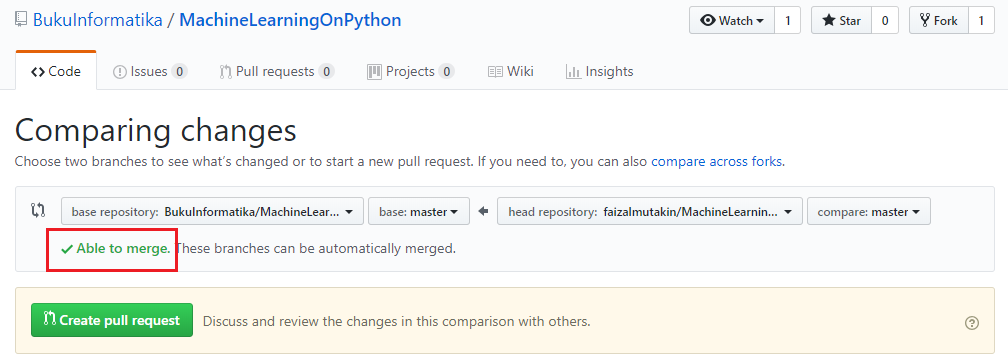
\includegraphics[width=1\textwidth]{figures/1.PNG}
		\caption{Gambar new pull requesh}
		\label{labelgambar1}
		\end{figure}	 
\end{enumerate}


\chapter{Contoh Laporan Harian dan Mingguan Menggunakan Tabel}
\chapter{Contoh Laporan Harian dan Mingguan}
\textbf{Contoh 1}
% Please add the following required packages to your document preamble:
% \usepackage[normalem]{ulem}
% \useunder{\uline}{\ul}{}
\begin{table}[]
\caption{Laporan Harian Tanggal 25 Februari 2018}
\label{tab:lh250219}
\begin{tabular}{|l|l|l|}
\hline
\textbf{No} & \multicolumn{1}{c|}{\textbf{Kategori}} & \multicolumn{1}{c|}{\textbf{Keterangan}} \\ \hline
1 & Dedikasi & - \\ \hline
2 & Produktifitas & \begin{tabular}[c]{@{}l@{}}a. Membuat repositori Modul Praktikum kelas Pemrograman III\\     Kelas 2A, 2B, dan 2C di organisasi pemograman-iii.\end{tabular} \\
 &  & b. Mengintal python, pip, anaconda, dan jupiter dari Udemy. \\
 &  & \begin{tabular}[c]{@{}l@{}}c. Melakukan merge pull request di pemograman-iii/praktikum\_2a,\\    dari \#1, \#3, \#4, \#7, \#8, \#9, \#10, \#12, \#13, dan \#14.\end{tabular} \\ \hline
3 & Integritas & able to merge/has no conflict \\ \hline
4 & Disiplin & Jam Datang : 07.07 WIB \\
 &  & Jam Pulang : 16.20 WIB \\ \hline
5 & Loyalitas & \begin{tabular}[c]{@{}l@{}}Membersihkan dan merapihkan meja kerja, dan mengecek AC\\ di pagi dan sore hari.\end{tabular} \\ \hline
\end{tabular}
\end{table}

% Please add the following required packages to your document preamble:
% \usepackage[normalem]{ulem}
% \useunder{\uline}{\ul}{}
\begin{table}[]
\caption{Laporan Harian Tanggal 26 Februari 2018}
\label{tab:lh260219}
\begin{tabular}{|l|l|l|}
\hline
\textbf{No} & \multicolumn{1}{c|}{\textbf{Kategori}} & \multicolumn{1}{c|}{\textbf{Keterangan}} \\ \hline
1 & Dedikasi & - \\ \hline
2 & Produktifitas & a. Membuat repositori Modul Praktikum kelas Kecerdasan Buatan. \\
 &  & b. Mendata dan menilai tugas 1 kelas 2A-Pemrograman III. \\
 &  & \begin{tabular}[c]{@{}l@{}}c. Membimbing Fadila, Lusia, dan Rahmi Roza kelas 3C untuk \\     tugas Kecerdasan Buatan.\end{tabular} \\ \hline
3 & Integritas & able to merge/has no conflict \\ \hline
4 & Disiplin & Jam Datang : 08.30 WIB \\
 &  & Jam Pulang : 16.30 WIB \\ \hline
5 & Loyalitas & \begin{tabular}[c]{@{}l@{}}Membersihkan dan merapihkan meja kerja, dan mengecek AC\\ di pagi dan sore hari.\end{tabular} \\ \hline
\end{tabular}
\end{table}

\begin{table}[]
\caption{Laporan Harian Tanggal 27 Februari 2019}
\label{tab:lh270219}
\begin{tabular}{|l|l|l|}
\hline
\textbf{No} & \multicolumn{1}{c|}{\textbf{Kategori}} & \multicolumn{1}{c|}{\textbf{Keterangan}} \\ \hline
1 & Dedikasi & bukuinformatika/flask \#10 \\ \hline
2 & Produktifitas & a.Mendata dan menilai tugas kelas 3C-Kecerdasan Buatan. \\
 &  & b.Membimbing anak kelas 3C untuk tugas Kecerdasan Buatan. \\
 &  & c. Mengkoordinasi tugas kontribusi anak kelas. \\ \hline
3 & Integritas & able to merge/has no conflict \\ \hline
4 & Disiplin & Jam Datang : 08.50 WIB \\
 &  & Jam Pulang : 17.30 WIB \\ \hline
5 & Loyalitas & \begin{tabular}[c]{@{}l@{}}Membersihkan dan merapihkan meja kerja, dan mengecek AC\\ di pagi dan sore hari.\end{tabular} \\ \hline
\end{tabular}
\end{table}

\begin{table}[]
\caption{Laporan Harian Tanggal 28 Februari 2019}
\label{tab:lh280219}
\begin{tabular}{|l|l|l|}
\hline
\textbf{No} & \multicolumn{1}{c|}{\textbf{Kategori}} & \multicolumn{1}{c|}{\textbf{Keterangan}} \\ \hline
1 & Dedikasi & BukuInformatika/flask \#12 \\ \hline
2 & Produktifitas & \begin{tabular}[c]{@{}l@{}}a. Evaluasi mingguan dan sosialisasi format baru penilaian peserta\\     internship II di IRC dan Prodi.\end{tabular} \\
 &  & \begin{tabular}[c]{@{}l@{}}b. Memeriksa lembar jawaban UAS GIS kelas 3C dan Arkom\\     kelas 1C.\end{tabular} \\
 &  & c. Menginput nilai UAS kelas 1C, 3A, 3B, dan 3C di google docs. \\
 &  & \begin{tabular}[c]{@{}l@{}}d. Mengkoordinir mahasiswa untuk tugas kontribusi pembuatan cover,\\     pencetakan, sampai pendistribusian buku di Grup Whatsapp.\end{tabular} \\
 &  & \begin{tabular}[c]{@{}l@{}}e. Memeriksa tugas kecerdasan buatan kelas 3C serta menginput nilai\\     ke google docs atas nama Fadila, Lusia Violita Aprilian, dan Rahmi.\end{tabular} \\ \hline
3 & Integritas & able to merge/has no conflict \\ \hline
4 & Disiplin & Jam Datang : 07.55 WIB \\
 &  & Jam Pulang : 17.00 WIB \\ \hline
5 & Loyalitas & \begin{tabular}[c]{@{}l@{}}Menyapu, membersihkan dan merapihkan meja, mencuci gelas nomor 6,\\ dan mengecek AC di pagi dan sore hari.\end{tabular} \\ \hline
\end{tabular}
\end{table}

\begin{table}[]
\caption{Laporan Harian Tanggal 1 Maret 2019}
\label{tab:lh010319}
\begin{tabular}{|l|l|l|}
\hline
\textbf{No} & \multicolumn{1}{c|}{\textbf{Kategori}} & \multicolumn{1}{c|}{\textbf{Keterangan}} \\ \hline
1 & Dedikasi &  \\ \hline
2 & Produktifitas & \begin{tabular}[c]{@{}l@{}}a. Mengerjakan Soal Toefl Pre-Test 2 (Computer Based)\\     Skor Toefl: 55\end{tabular} \\
 &  & b. Mendata skor toefl peserta Internship II di IRC. \\
 &  & c. Memeriksa pull request di laporanirc/2019. \\ \hline
3 & Integritas & able to merge/has no conflict \\ \hline
4 & Disiplin & Jam Datang : 07.39 WIB \\
 &  & Jam Pulang : 14.20 WIB \\ \hline
5 & Loyalitas & \begin{tabular}[c]{@{}l@{}}Menyapu, membersihkan dan merapihkan meja, membeli\\ sabun dan spons cuci piring, dan mengecek AC di pagi\\ dan sore hari.\end{tabular} \\ \hline
\end{tabular}
\end{table}

\section{Penilaian Mingguan}

\begin{table}[h]
\centering
\caption{Nilai Minggu ke-1}
\label{tab:nm01}
\begin{tabular}{|c|c|c|}
\hline
\textbf{No} & \textbf{Kategori} & \textbf{Poin} \\ \hline
1 & Dedikasi & 1 \\ \hline
2 & Produktifitas & 3 \\ \hline
3 & Integritas & 3 \\ \hline
4 & Disiplin & 3 \\ \hline
5 & Loyalitas & 3 \\ \hline
 & \textbf{Total Poin} & 13 \\ \hline
\end{tabular}
\end{table}





\chapter{Contoh Laporan Harian dan Mingguan Menggunakan Penomoran}
\begin{enumerate}
\item \textbf{Tugas Harian tanggal 17/01/2019}
\begin{enumerate}
\item Membersihkan ruang IRC
\item Diskusi mengenai penataan ulang ruang IRC
\end{enumerate}

\item \textbf{Tugas Harian tanggal 18/01/2019}
\begin{enumerate}
\item Membersihkan ruang IRC
\item Diskusi mengenai rancangan ruang IRC
\item Diskusi mengenai barang yang harus ditambahkan di ruang IRC
\item Membuat artikel untuk bahan majalah D4 TI
\end{enumerate}

\item \textbf{Tugas Harian tanggal 21/01/2019}
\begin{enumerate}
\item Mencari artikel untuk bahan majalah
\item Diskusi tentang perancangan ruang sidang di IRC
\end{enumerate}

\item \textbf{Tugas Harian tanggal 30/02/2019}
\begin{enumerate}
\item Mendata buku yang akan dipindahkan ke IRC
\end{enumerate}

\item \textbf{Tugas Harian tanggal 31/01/2019}
\begin{enumerate}
\item Memberi label pada buku untuk IRC
\item Memindahkan buku sumbangan ke IRC
\end{enumerate}

\item \textbf{Tugas Harian tanggal 01/02/2019}
\begin{enumerate}
\item Praktek github dengan Pak Rolly Maulana Awangga 
\end{enumerate}

\item \textbf{Tugas Harian tanggal 06/02/2019}
\begin{enumerate}
\item Membuat video pesan, kesan dan kritik untuk IRC
\end{enumerate}

\item \textbf{Tugas Harian tanggal 18/02/2019}
\begin{enumerate}
\item Memperhatikan tingkat 3 presentasi
\item Mengoreksi laporan tingkat 3 yang presentasi
\item Memeriksa revisian tutorial class diagram adik tingkat
\end{enumerate}

\item \textbf{Tugas Harian tanggal 25/02/2019}
\begin{enumerate}
\item Masuk Kelas Pemrograman III
\item Menginstal python, anaconda
\item Menambah materi udemy (commit 8b5991b08ef04a0c1581f5976017e7eab865c856)
\item Menambah materi di GIS2019 (commit f1535f03dd64c09ddba50f68371ec04b878846e9, commit 0ff764471c1cefd7e6b20d81027d7d810c1343d5, commit c054dcbfa03e9a2d9ef56f3302d8f0854840d758)
\item Memeriksa tugas Pemrograman III kelas 2b (1174034 Ichsan Hizman Hardy, 1174050 Dika Sukma Pradana, 1174042 Faisal Najib Abdullah, 1174035 Luthfi Muhammad Nabil, 1174040 Hagan Rowlenstino, 1174043 Irvan Rizkiansyah, 1174063 Muhamad Iqbal Panggabean, 1174057 Alit fajar Kurniawan, 1174059 Kevin Natanael Nainggolan)
\end{enumerate}

\textbf{Dedikasi}
\begin{enumerate} 
\item  Menambah materi di GIS2019 (commit f1535f03dd64c09ddba50f68371ec04b878846e9, commit 0ff764471c1cefd7e6b20d81027d7d810c1343d5, commit c054dcbfa03e9a2d9ef56f3302d8f0854840d758)
\end{enumerate}

\textbf{Produktifitas}
\begin{enumerate}
\item Masuk Kelas Pemrograman III
\item Menginstal python, anaconda
\item Menambah materi udemy (commit 8b5991b08ef04a0c1581f5976017e7eab865c856
\item Menambah materi di GIS2019 (commit f1535f03dd64c09ddba50f68371ec04b878846e9, commit 0ff764471c1cefd7e6b20d81027d7d810c1343d5, commit c054dcbfa03e9a2d9ef56f3302d8f0854840d758)
\item Memeriksa tugas Pemrograman III kelas 2b (1174034 Ichsan Hizman Hardy, 1174050 Dika Sukma Pradana, 1174042 Faisal Najib Abdullah, 1174035 Luthfi Muhammad Nabil, 1174040 Hagan Rowlenstino, 1174043 Irvan Rizkiansyah, 1174063 Muhamad Iqbal Panggabean, 1174057 Alit fajar Kurniawan, 1174059 Kevin Natanael Nainggolan)
\end{enumerate}

\textbf{Integritas}
\begin{enumerate}
\item able to merge/has no conflict
\end{enumerate}

\textbf{Disiplin}
\begin{enumerate}
\item Jam Masuk : 08.40
\item Jam Keluar : 15.30
\end{enumerate}

\textbf{Loyalitas}
\begin{enumerate}
\item Mengecek AC saat datang dan pulang dari IRC
\item Merapihkan meja dan kursi saat pulang dari IRC
\item Merapihkan CPU ke lemari
\item Merapihkan banner ke lemari
\item Menjaga peralatan yang ada di IRC  
\end{enumerate}

\item \textbf{Tugas Harian tanggal 26/02/2019}
\begin{enumerate}
\item Masuk kelas Kecerdasan Buatan
\item Membuat repository tugas kecerdasan buatan kelas 3c
\item Menginput nilai tugas Pemrograman III kelas 2b
\item Menambah materi GIS 2019, commit d97e9474087a3faca296fef82e9e7503345ac45e
\end{enumerate}

\textbf{Dedikasi}
\begin{enumerate}
\item Menambah materi GIS 2019, commit d97e9474087a3faca296fef82e9e7503345ac45e
\end{enumerate}

\textbf{Produktifitas}
\begin{enumerate}
\item Masuk kelas Kecerdasan Buatan
\item Membuat repository tugas kecerdasan buatan kelas 3c
\item Menginput nilai tugas Pemrograman III kelas 2b
\item Menambah materi GIS 2019, commit d97e9474087a3faca296fef82e9e7503345ac45e
\end{enumerate}

\textbf{Integritas}
\begin{enumerate}
\item able to merge/has no conflict
\end{enumerate}

\textbf{Disiplin}
\begin{enumerate}
\item Jam Masuk : 08.40
\item Jam Keluar : 15.30
\end{enumerate}

\textbf{Loyalitas}
\begin{enumerate}
\item Mengecek AC saat datang dan pulang dari IRC
\item Merapihkan kursi saat pulang dari IRC
\item Menjaga peralatan yang ada di IRC
\end{enumerate}

\item \textbf{Tugas Harian tanggal 27/02/2019}
\begin{enumerate}
\item Mangecek tugas kecerdasan buatan kelas 3c
\item Menginput nilai tugas kecerdasan buatan kelas 3c
\item Memberikan arahan dan hukuman bagi mahasiswa yang tidak melakukan pull request, tidak membenarkan conflict dan tidak mengerjakan tugas Pemrograman III kelas 2b
\item Menginput nilai tugas Pemrograman III kelas 2b (1174034 Ichsan Hizman Hardy, 1174050 Dika Sukma Pradana, 1174042 Faisal Najib Abdullah, 1174035 Luthfi Muhammad Nabil, 1174040 Hagan Rowlenstino, 1174043 Irvan Rizkiansyah, 1174063 Muhamad Iqbal Panggabean, 1174057 Alit fajar Kurniawan, 1174059 Kevin Natanael Nainggolan)
\item Menambah materi GIS 2019, commit d97e9474087a3faca296fef82e9e7503345ac45e
\item Menandatangani acc tutorial membuat class diagram (Ajis Trigunawan 1164031 dan Wildan Khaustara W 1164058)
\item Memeriksa dan memberi revisian jurnal projek II Ajis Trigunawan 1164031
\end{enumerate}

\textbf{Dedikasi}
\begin{enumerate}
\item Menambah materi GIS 2019, commit d97e9474087a3faca296fef82e9e7503345ac45e
\end{enumerate}

\textbf{Produktifitas}
\begin{enumerate}
\item Masuk kelas Kecerdasan Buatan
\item Membuat repository tugas kecerdasan buatan kelas 3c
\item Menginput nilai tugas Pemrograman III kelas 2b (1174034 Ichsan Hizman Hardy, 1174050 Dika Sukma Pradana, 1174042 Faisal Najib Abdullah, 1174035 Luthfi Muhammad Nabil, 1174040 Hagan Rowlenstino, 1174043 Irvan Rizkiansyah, 1174063 Muhamad Iqbal Panggabean, 1174057 Alit fajar Kurniawan, 1174059 Kevin Natanael Nainggolan)
\item Menambah materi GIS 2019, commit d97e9474087a3faca296fef82e9e7503345ac45e
\item Menandatangani acc tutorial membuat class diagram (Ajis Trigunawan 1164031 dan Wildan Khaustara W 1164058)
\item Memeriksa dan memberi revisian jurnal projek II Ajis Trigunawan 1164031
\end{enumerate}

\textbf{Integritas}
\begin{enumerate}
\item able to merge/has no conflict
\end{enumerate}

\textbf{Disiplin}
\begin{enumerate}
\item Jam Masuk : 08.40
\item Jam Keluar : 15.30
\end{enumerate}

\textbf{Loyalitas}
\begin{enumerate}
\item Mengecek AC saat datang dan pulang dari IRC
\item Merapihkan kursi saat pulang dari IRC
\item Menjaga peralatan yang ada di IRC
\end{enumerate}

\item \textbf{Tugas Harian tanggal 27/02/2019}
\begin{enumerate}
\item Mangecek tugas kecerdasan buatan kelas 3c (Andi Muh Aslam 1164064 dan Aip Suprapto Munari 1164063)
\item Menginput nilai tugas kecerdasan buatan kelas 3c (Andi Muh Aslam 1164064 dan Aip Suprapto Munari 1164063)
\item Memberikan arahan dan hukuman bagi mahasiswa yang tidak melakukan pull request, tidak membenarkan conflict dan tidak mengerjakan tugas Pemrograman III kelas 2b
\item Menambah gambar pada Materi GIS (menambahkan gambar \#11) 
\end{enumerate}

\textbf{Dedikasi}
\begin{enumerate}
\item Menambah gambar pada Materi GIS (menambahkan gambar \#11) 
\end{enumerate}

\textbf{Produktifitas}
\begin{enumerate}
\item Mangecek tugas kecerdasan buatan kelas 3c (Andi Muh Aslam 1164064 dan Aip Suprapto Munari 1164063)
\item Menginput nilai tugas kecerdasan buatan kelas 3c (Andi Muh Aslam 1164064 dan Aip Suprapto Munari 1164063)
\item Memberikan arahan dan hukuman bagi mahasiswa yang tidak melakukan pull request, tidak membenarkan conflict dan tidak mengerjakan tugas Pemrograman III kelas 2b
\item Menambah gambar pada Materi GIS (menambahkan gambar \#11) 
\end{enumerate}

\textbf{Integritas}
\begin{enumerate}
\item able to merge/has no conflict
\end{enumerate}

\textbf{Disiplin}
\begin{enumerate}
\item Jam Masuk : 08.40
\item Jam Keluar : 15.30
\end{enumerate}

\textbf{Loyalitas}
\begin{enumerate}
\item Mengecek AC saat datang dan pulang dari IRC
\item Merapihkan kursi saat pulang dari IRC
\item Menjaga peralatan yang ada di IRC
\end{enumerate}


\item \textbf{Tugas Harian tanggal 28/02/2019}
\begin{enumerate}
\item Evaluasi mingguan dengan Pak Rolly Maulana Awangga
\item Menilai hasil UAS kelas 1C, 3A dan 3C
\item Menata ulang ruang IRC
\item Memeriksa tugas kelas Kecerdasan Buatan 3C Andi Muh Aslam 1164064, hari2 \#3 dan  Aip Suprapto Munari 1164063  (tugas masih conflict)
\item Menginput nilai tugas Kecerdasan Buatan kelas 3C Andi Muh Aslam 1164064 dan Aip Suprapto Munari 1164063 
\item Menambah materi sumber sumber data geospasial \#13
\end{enumerate}

\textbf{Dedikasi}
\begin{enumerate}
\item Menambah materi sumber sumber data geospasial \#13
\end{enumerate}

\textbf{Produktifitas}
\begin{enumerate}
\item Evaluasi mingguan dengan Pak Rolly Maulana Awangga
\item Menilai hasil UAS kelas 1C, 3A dan 3C
\item Menata ulang ruang IRC
\item Memeriksa tugas kelas Kecerdasan Buatan 3C Andi Muh Aslam 1164064, hari2 \#3 dan  Aip Suprapto Munari 1164063  (tugas masih conflict)
\item Menginput nilai tugas Kecerdasan Buatan kelas 3C Andi Muh Aslam 1164064 dan Aip Suprapto Munari 1164063 
\end{enumerate}

\textbf{Integritas}
\begin{enumerate}
\item able to merge/has no conflict
\end{enumerate}

\textbf{Disiplin}
\begin{enumerate}
\item Jam Masuk : 08.40
\item Jam Keluar : 17.30
\end{enumerate}

\textbf{Loyalitas}
\begin{enumerate}
\item Mengecek AC saat datang dan pulang dari IRC
\item Merapihkan kursi saat pulang dari IRC
\item Menjaga peralatan yang ada di IRC
\item Mengatur ulang ruang IRC 
\end{enumerate}

\item \textbf{Tugas Harian tanggal 01/03/2019}
\begin{enumerate} 
\item Melakukan pre test TOEFL 
\item Memberi tahu kelas 3B untuk mencantumkan sitasi dan sumber di daftar pustaka mengenai materi GIS
\item menambah materi dan gambar mengenai sumber sumber data geospasial \#16
\end{enumerate}

\textbf{Dedikasi}
\begin{enumerate}
\item menambah materi dan gambar mengenai sumber sumber data geospasial \#16
\end{enumerate}

\textbf{Produktifitas}
\begin{enumerate}
\item Melakukan pre test TOEFL 
\item Memberi tahu kelas 3B untuk mencantumkan sitasi dan sumber di daftar pustaka mengenai materi GIS
\item menambah materi dan gambar mengenai sumber sumber data geospasial \#16
\end{enumerate}

\textbf{Integritas}
\begin{enumerate}
\item able to merge/has no conflict
\end{enumerate}


\textbf{Disiplin}
\begin{enumerate}
\item Jam Masuk : 08.40
\item Jam Keluar : 11.40 (Dikarenakan ada sosialisasi INTERNSHIP II)
\end{enumerate}


\textbf{Loyalitas}
\begin{enumerate}
\item Mengecek AC saat datang dan pulang dari IRC
\item Menjaga peralatan yang ada di IRC
\item Merapihkan kursi setelah pulamg dari IRC
\item Mengelap meja pribadi
\item Menyapu dan merapihkan area sidang IRC
\item Membersihkan lemari buku 
\end{enumerate}

\item \textbf{Tugas Harian tanggal 04/03/2019}
\begin{enumerate}
\item Menambah gambar dan materi mengenai sumber sumber data geospasial \#17
\item Masuk kelas Pemrograman 3 
\item Diskusi mengenai INTERNSHIP II bersama Bapak Rolly Maulana Awangga
\item Membuat orgnanisasi INTERNSHIPD4TI di github
\item Kontribusi pada repository PPK (template \#1, merapihkan dan menambah contoh laporan harian dan mingguan \#8)
\item Menambah materi deep learning computer vision \#3
\item Membersihkan meja pribadi
\item Membersihkan area sidang 
\end{enumerate}

\textbf{Dedikasi}
\begin{enumerate}
\item Menambah gambar dan materi mengenai sumber sumber data geospasial \#17
\item Kontribusi pada repository PPK (template \#1, merapihkan dan menambah contoh laporan harian dan mingguan \#8)
\item Menambah materi deep learning computer vision \#3
\end{enumerate}

\textbf{Produktifitas}
\begin{enumerate}
\item Menambah gambar dan materi mengenai sumber sumber data geospasial \#17
\item Masuk kelas Pemrograman 3 
\item Diskusi mengenai INTERNSHIP II bersama Bapak Rolly Maulana Awangga
\item Membuat orgnanisasi INTERNSHIPD4TI di github
\item Kontribusi pada repository PPK (template \#1, merapihkan dan menambah contoh laporan harian dan mingguan \#8)
\item Menambah materi deep learning computer vision \#3
\item Membersihkan meja pribadi
\item Menyapu dan merapihkan area sidang 
\end{enumerate}

\textbf{Integritas}
\begin{enumerate}
\item able to merge/has no conflict
\end{enumerate}


\textbf{Disiplin}
\begin{enumerate}
\item Jam Masuk : 08.40
\item Jam Keluar : 17.40
\end{enumerate}


\textbf{Loyalitas}
\begin{enumerate}
\item Mengecek AC saat datang dan pulang dari IRC
\item Menjaga peralatan yang ada di IRC
\item Merapihkan kursi setelah pulamg dari IRC
\item Mengelap meja pribadi
\item Menyapu dan merapihkan area sidang IRC
\item Membersihkan meja pribadi
\end{enumerate}
\end{enumerate}

\section{Score Mingguan dari tanggal 25/02/2019 sampai 01/03/2019}
Total score mingguan adalah 15 keterangan seperti pada Tabel \ref{table:scoremingguan}.
\begin{table}[!ht]
\centering
\begin{tabular}{ |c|c|c|c|c|c|c|c|c|c| }
\hline
Kategori & Keterangan Nilai \\
\hline
Dedikasi & 3 \\
\hline
Produktif & 3 \\
\hline
Integritas & 3 \\
\hline
Disiplin & 3 \\
\hline
Loyalitas & 3 \\
\hline
\end{tabular}
\caption{Tabel Score Mingguan}
\label{table:scoremingguan}
\end{table}









\bibliographystyle{IEEEtran} 
%\def\bibfont{\normalsize}
\bibliography{references}


%%%%%%%%%%%%%%%
%%  The default LaTeX Index
%%  Don't need to add any commands before \begin{document}
\printindex

%%%% Making an index
%% 
%% 1. Make index entries, don't leave any spaces so that they
%% will be sorted correctly.
%% 
%% \index{term}
%% \index{term!subterm}
%% \index{term!subterm!subsubterm}
%% 
%% 2. Run LaTeX several times to produce <filename>.idx
%% 
%% 3. On command line, type  makeindx <filename> which
%% will produce <filename>.ind 
%% 
%% 4. Type \printindex to make the index appear in your book.
%% 
%% 5. If you would like to edit <filename>.ind 
%% you may do so. See docs.pdf for more information.
%% 
%%%%%%%%%%%%%%%%%%%%%%%%%%%%%%

%%%%%%%%%%%%%% Making Multiple Indices %%%%%%%%%%%%%%%%
%% 1. 
%% \usepackage{multind}
%% \makeindex{book}
%% \makeindex{authors}
%% \begin{document}
%% 
%% 2.
%% % add index terms to your book, ie,
%% \index{book}{A term to go to the topic index}
%% \index{authors}{Put this author in the author index}
%% 
%% \index{book}{Cows}
%% \index{book}{Cows!Jersey}
%% \index{book}{Cows!Jersey!Brown}
%% 
%% \index{author}{Douglas Adams}
%% \index{author}{Boethius}
%% \index{author}{Mark Twain}
%% 
%% 3. On command line type 
%% makeindex topic 
%% makeindex authors
%% 
%% 4.
%% this is a Wiley command to make the indices print:
%% \multiprintindex{book}{Topic index}
%% \multiprintindex{authors}{Author index}

\end{document}

